\documentclass[letterpaper]{article}

\usepackage[utf8]{inputenc}
\usepackage{amsmath}
\usepackage{hyperref}
\usepackage{graphicx}
\usepackage{comment}

\graphicspath{ {./images/} }

\title{A DSL for writing safer string manipulation functions in C}
\author{Michael Flanders}
\date{December 16, 2020}

%You can skip explaining the state of the art (i.e., how the problem is solved today).
%Instead, make sure to include a description of your language. Ideally,
%  you present a language tutorial using your previously selected examples. 
%When explaining your design, refer back to the architecture of DSL
%  implementations, similarly to how we asked you about the FFTW architecture
%  in the reading homework. 
%Please make your design description point to the relevant lines of your implementation.
%  Ideally, your doc will include links to the range of code in your github repo. 
%Please share the repo with the user rbodik. 
%Include the answers to the questions from the last slide.
%Please add the answer to the question "What knowledge or skill would have helped you
%  be more successful with the project."  The answers will help us in further upgrading
%  the course. 

\begin{document}
\maketitle

% Overview of project
% what was proposed initially vs what made it into code at the end
% Overview of the sections

\section{Domain analysis}

% vs runtime checks vs static analyzers vs SE
% Sample problems from slides
% Easy, medium, hard samples

\section{Language description}

% Overview
% Paradigm, immutability, boundedness
% Language constructs, operators
% Ranges, subranges
% For loops

\section{Design and decisions}

\begin{figure}[h]
  \centering
  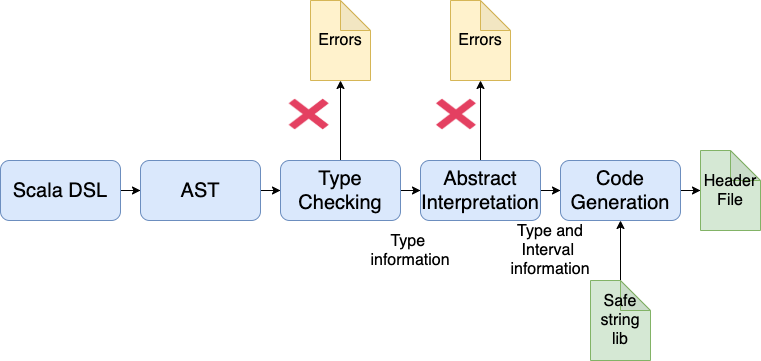
\includegraphics[width=\textwidth]{architecture.png}
  \caption{Diagram of the compiler pipeline}
  \label{fig:pipeline}
\end{figure}

\begin{figure}[h]
  \centering
  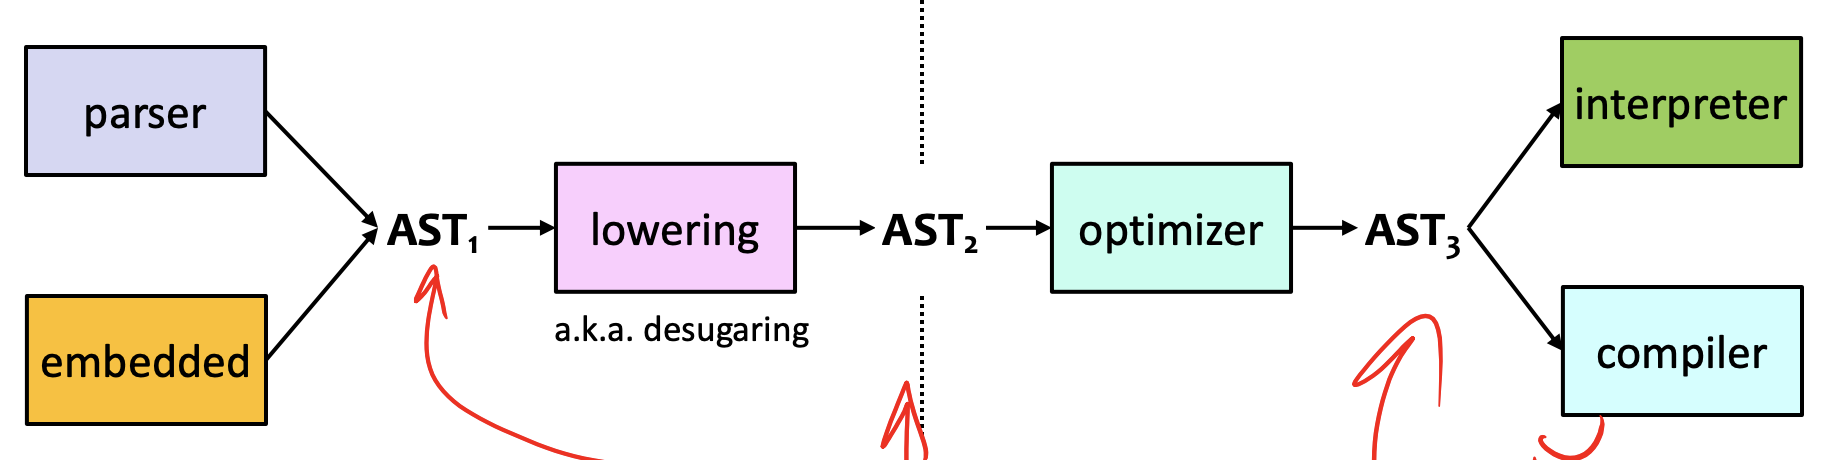
\includegraphics[width=\textwidth]{modern-compiler-pipeline.png}
  \caption{Diagram of the compiler pipeline. (Screenshot from the marked up lecture slides)}
  \label{fig:mdnpipeline}
\end{figure}

% Overview
% Lexer/parser vs fluent-syntax/call-chaining
% Typechecker
%  the basics and some of the other checks:
%   no recursion
%   ranges well formed (lower bound <=  upper bound)
%  monadic, pretty proud of this. Lots of Option,Either mixed, wished it was cleaner still
% Abstract interpreter
%  abstract domain is intervals
%  didn't finish, couldn't get 
%  everything is bounded, all loops end => widening and narrowing are optimizations
%   not necessities, so easier to just build abs int, act like normal interpreter and
%   just ride loops out
%  vs symbolic execution
%   ended up seeming like more work getting the integer semantics symbolic but
%   i think it would've ended up just as precise but a little slower
% Code generation
%  Didn't finish this, couldn't get:
%    most of the string functions written
%    freeing of complicated data
%     2 solutions, copy/dupe all strings from iters or some kind of analysis
%  the safe string library
%    static inlined
%    could get the code gen to just write one C function but it ended up looking messy,
%     developers might not trust it

\section{Discussion}

% Answer the questions from the last slide (of the template?)
%  What are you proud of? A neat trick in the design or implementation
%    of your language.
%
%  Mistakes describe a mistak you made, e.g., a construct you think will confuse programmers
%
%  What we would do differently
%    Give the lessons you learnt in this project, if you have to start again, what would you do differently?
%
% "What knowledge or skill would have helped you be more successful in the project?"
%
%   Wish we got some deeper monadic/parametrized interpreter coding homeworks. I did the
%   all of the monads for functional programming and essence of fp examples, but they only
%   touched on one monad at a time and really simple semantics. I ended up only really underst
%   standing monad transformers and free monads 1-2 days before the final presentation, so I
%   wish I knew more about engineering an interpreter so I could've used this. Contrast w/
%   FFTW. example is checkStmt for For in typechecker
%   

\end{document}
